\documentclass[11pt,a4paper]{article}

\usepackage{pdflscape}
\usepackage{graphicx}
\usepackage[utf8]{inputenc}
\usepackage[czech]{babel}
\usepackage[IL2]{fontenc}
\usepackage[unicode]{hyperref}
\usepackage{times}
\usepackage{amsmath, amsthm, amssymb}
\usepackage{algorithm}
\usepackage{algorithmic}
\usepackage{multirow}
\graphicspath{ {images/} }

\usepackage[left=2cm,top=3cm,text={17cm,24cm}]{geometry}

\floatname{algorithm}{Algoritmus:}
\renewcommand{\algorithmicrequire}{\textbf{Input:}}
\renewcommand{\algorithmicensure}{\textbf{Output:}}



\begin{document}

\begin{titlepage}
    \begin{center}
        \textsc{\Huge Fakulta informačních technologii\\\vspace{0.4em}
        vysoké učení technické v Brně}\\
        \vspace{\stretch{0.382}}
        {\LARGE Typografie a publikování -- 3. projekt\\\vspace{0.3em}
       Tabulky a obrázky}c
        \vspace{\stretch{0.618}}
    \end{center}
    \begin{flushleft}
        \today
        \hfill
        Pavel Yadlouski (xyadlo00)
    \end{flushleft}
\end{titlepage}

\newpage

\section{Úvodní strana}
Název práce umístěte do zlatého řezu a nezapomeňte uvést dnešní datum a vaše jméno a příjmení.

\section{Tabulky}

Pro sázení tabulek můžeme použít buď prostředí \texttt{tabbing} nebo prostředí \texttt{tabular}.
Prostøedí tabbing

\subsection{Prostředí \texttt{tabbing}}

Při použití \texttt{tabbing} vypadá následovně:

\begin{tabbing}
    \textbf{Ovoce }\hspace{1.5cm} \=   \textbf{Cena } \hspace{0.1cm} \= \textbf{Množství}\\ 
    Jablka \> 25,90 \> 3 kg\\
    Hrušky \> 27.40 \> 2.5 kg \\
    Vodní melouny \> 35,00 \> 1 kus
\end{tabbing}
Toto prostředí se dá použít pro sázení algoritmů, ovšem vhodnější je použit prostředí \texttt{algorithm} nebo \texttt{algorithm2e} (viz sekce 3).

\subsection{Prostředí \texttt{tabular}}
Další možnost, jak vytvořit tabulku, je použít prostředí \texttt{tabular}. Tabulky pak budou vypadat takto\footnote{Kdyby byl problem s \texttt{cline}, zkuste se podívat třeba sem: \url{http://www.abclinuxu.cz/tex/poradna/show/325037}}:


\begin{table}[h]
	 \catcode`\-=12
    \begin{center}
        \begin{tabular}{|l|l|l|}
        \hline
              & \multicolumn{2}{c|}{\textbf{Cena}}\\ 
              \cline{2-3}
         \textbf{Měna} & \textbf{prodej} & \textbf{nakup} \\ 
        \hline
        EUR & 25.615 & 27.20\\
        GBP & 29.899 & 31.80\\
        USD & 22.571 & 25,51\\
        \hline
        \end{tabular}
        \caption{Tabulka kurzů k dnešnímu dni}
        \label{tab:tab1}
    \end{center}
\end{table}
\begin{table}[h]
	\catcode`\-=12
	%first tabel	
	\begin{center}
		\begin{tabular}{|l|l|}
			\hline		
			A & $\neg$A \\
		 	\hline
	 		\textbf{P} & N \\
	 		\hline
	 		\textbf{O} & o \\
			\hline
		 	\textbf{X} & X \\
		 	\hline
		 	\textbf{N} & N \\
	 		\hline
		\end{tabular}
		%second tabel		
		\begin{tabular}{|l|l|l|l|l|l|}
			\hline			
			\multicolumn{2}{|c|}{\multirow{2}{*}{$A \wedge B$}} & \multicolumn{4}{c|}{B} \\
			\cline{3-6}
		 	 \multicolumn{2}{|c|}{} & \textbf{P} & \textbf{O} & \textbf{X} & \textbf{N} \\  	
			\hline		 
			\multirow{4}{*}{\textbf{A}} & \textbf {P} & P & O & X & N  \\
			\cline{2-6}		 
		 	& \textbf{O} & O & O & N & N \\ 
			\cline{2-6}		
		 	& \textbf{X} & X & N & X & N \\
			\cline{2-6}
		 	& \textbf{N} & N & N & N & N \\
			\hline		
		\end{tabular}
		%thread tabel
		\begin{tabular}{|l|l|l|l|l|l|}
			\hline			
			\multicolumn{2}{|c|}{\multirow{2}{*}{$A \vee B$}} & \multicolumn{4}{c|}{B} \\
			\cline{3-6}
			\multicolumn{2}{|c|}{}& \textbf{P} & \textbf{O} & \textbf{X} & \textbf{N} \\  	
			\hline		 
			\multirow{4}{*}{\textbf{A}} & \textbf {P} & P & P & P & P  \\
			\cline{2-6}		 
		 	& \textbf{O} & P & O & P & O \\ 
			\cline{2-6}		
			& \textbf{X} & P & P & X & X \\
			\cline{2-6}
			& \textbf{N} & P & O & X & N \\
			\hline		
		\end{tabular}
		%fourth tabel
		\begin{tabular}{|l|l|l|l|l|l|}
			\hline			
			\multicolumn{2}{|c|}{\multirow{2}{*}{$A\rightarrow B$}} & \multicolumn{4}{c|}{B} \\
		\cline{3-6}
		 \multicolumn{2}{|c|}{}& \textbf{P} & \textbf{O} & \textbf{X} & \textbf{N} \\  	
		\hline		 
		\multirow{4}{*}{\textbf{A}} & \textbf {P} & P & O & X & N  \\
		\cline{2-6}		 
		 & \textbf{P} & P & O & P & O \\
		\cline{2-6}		
		 & \textbf{P} & P & P & X & X \\
		\cline{2-6}
		 & \textbf{P} & P & P & P & P \\
		\hline		
		\end{tabular}		
		
	\end{center}
	\caption{Protože Kleeneho trojhodnotová logika už je ``zastaralá``, uvádíme si zde příklad čtyřhodnotové logiky}
	\label{tab:tab2}
\end{table}



\newpage
\section{Algoritmy}
Pokud budete chtít vysázet algoritmus, můžete použít prostředí \texttt{algorithm}\footnote{Pro nápovědu, jak zacházet z prostředím \texttt{algorithm}, můžete zkusit tuhle straáku: \url{http://ftp.cstug.cz/pub/tex/CTAN/macros/latex/contrib/algorithms/algorithms.pdf}} nebo \texttt{algorithm2e} \footnote{Pro \texttt{algorithm2e} zase tuhle: \url{http://ftp.cstug.cz/pub/tex/CTAN/macros/latex/contrib/algorithms/algorithms.pdf}}. Příklad použití prostředí \texttt{algorithm2e} viz Algoritmus 1.

\begin{algorithm}
	\caption{: FastSlam} 
	\begin{algorithmic}[1]
		\REQUIRE ($X_{t-1},u_t,z_t$ ) 
		\ENSURE $X_{t}$
		\STATE {$\overline{X} = X_t = 0$}
		\FOR {$k = 1$ to $M$}
			\STATE $x^{[k]} = sample\_motion\_model = (u_t, x^{[k]}_{t-1})$
			\STATE $w^{[k]}_t = measurement\_model (z_t, x^{[k]}_t, m_{t-1}) $
			\STATE $m^{[k]}_t = updated\_occupancy\_grid (z_t, x^{[k]}_t, m^{[k]}_{t-1}) $
			\STATE $\overline{X} = \overline{X} + \langle x^{[m]}_x, w^{[m]}_t \rangle $		
		\ENDFOR
		\FOR {$k = 1$ to $M$}
			\STATE draw $i$ with probability $\approx w^{[i]}_t$
			\STATE add $\langle x^{[k]}_x, m^{[k]}_t \rangle$ to $X_t$   		
		\ENDFOR
		\RETURN $X_t$
	\end{algorithmic}
	\label{alg:alg1}
\end{algorithm}

\section{Obrázky}
Do naišch článků můžeme samozřejmě vkládat obrázky. Pokud je obrázkem fotografie, můžeme klidně použít bitmapový soubor. Pokud by to ale mělo být nějaké schéma nebo něco podobného, je dobrým zvykem takovýto
obrázek vytvořit vektorově.

\begin{figure}[h!]
	\begin{center}
		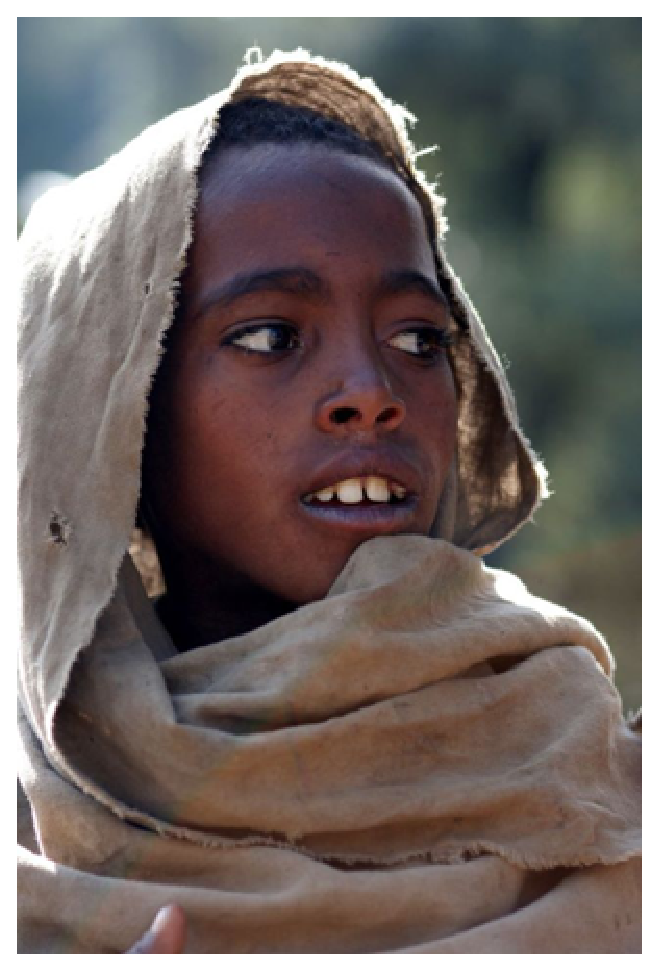
\includegraphics[scale=0.42]{etiopan.eps}
		\reflectbox{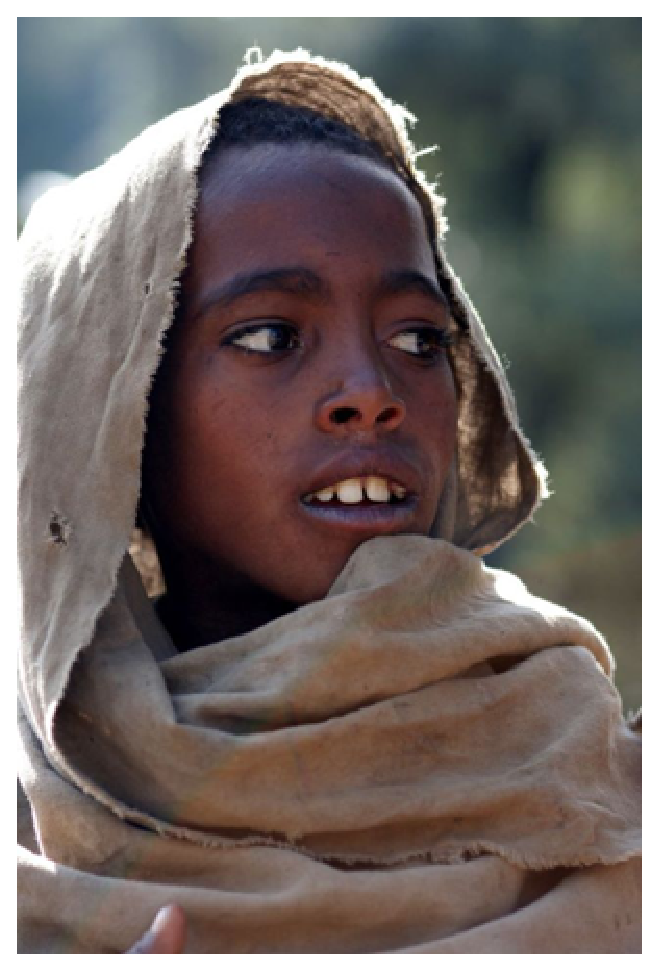
\includegraphics[scale=0.42]{etiopan.eps}}
		\caption{Malý Etiopánek a jeho bratříček} 
		\label{fig:etiopan}	
	\end{center}
\end{figure}

Rozdíl mezi vektorovým\ldots

\begin{figure}[h!]
	\begin{center}
		
\includegraphics[scale=0.42]{oniisan.eps}
		\caption{Vektorový obrázek} 
		\label{fig:on1}
	\end{center}
\end{figure}
\ldots bitmapovým obrázkem
\begin{figure}[h!]
	\begin{center}
		
\includegraphics[scale=0.67]{oniisan2.eps}
		\caption{Bitmapový obrázek} 
		\label{fig:on2}	
	\end{center}
\end{figure}

se projeví napřílad při zvětšení.

Odkazy (nejen ty) na obrázky \ref{fig:etiopan}, \ref{fig:on1} a \ref{fig:on2}, na tabulky \ref{tab:tab1} a \ref{tab:tab2} a také na algoritmus \ref{alg:alg1} jsou udělány pomocí křížových
odkazů. Pak je ovšem potřeba zdrojový soubor přeložit dvakrát.

Vektorové obrázky lze vytvořit i přímo v \LaTeX u, například pomocí prostředí \texttt{picture}.


\begin{landscape}
\begin{figure}[!ht]
	\setlength{\unitlength}{1cm}
	\fbox{
	\begin{picture}(23,15)
    	\put(2,1){\line(1,0){10}}
    	\put(2,1){\line(0,1){9}}
    	\put(2,10){\line(1,0){10}}
    	\put(12,10){\line(0,-1){9}}
		\put(2,1.5){\line(1,0){10}}    	
    	%roof
		\put(2,10){\line(5,4){5}}		
		\put(12,10){\line(-5,4){5}}
		\put(2.1,10){\line(5,4){4.9}}		
		\put(11.9,10){\line(-5,4){4.9}}	
		\put(7,12){\circle{3}}			
		%second flor
		\put(2,5.95){\line(1,0){10}}
		\put(2,6.05){\line(1,0){10}}
		%door on balkon		
		\put(9,6){\line(0,1){3}}
		\put(11,6){\line(0,1){3}}
		\put(9,9){\line(1,0){2}}
		%windows on balkon
		\put(6,7){\line(0,1){2}}
		\put(6,7){\line(1,0){2}}		
		\put(8,7){\line(0,1){2}}
		\put(6,9){\line(1,0){2}}
		\put(7,7){\line(0,1){2}}
		\put(6,8){\l`ine(1,0){2}}
		
		\put(3,7){\line(0,1){2}}
		\put(3,7){\line(1,0){2}}		
		\put(5,7){\line(0,1){2}}
		\put(3,9){\line(1,0){2}}
		\put(4,7){\line(0,1){2}}
		\put(3,8){\line(1,0){2}}
		%railing
		\multiput(2.5,6)(1,0){10}{\line(0,1){1.6}}
		\multiput(2.55,6)(1,0){10}{\line(0,1){1.6}}	
		\multiput(2.6,6)(1,0){10}{\line(0,1){1.6}}	
		\put(2,7.5){\line(1,0){10}}
		\put(2,7.55){\line(1,0){10}}
		\put(2,7.6){\line(1,0){10}}
			
		%door		
		\put(3,1){\line(0,1){4}}		
		\put(5,1){\line(0,1){4}}	
		\put(3,5){\line(1,0){2}}	
		\put(4.7,3.1){\circle{0.2}}
		%window on door
		\put(4,4){\circle{1}}		
		%oval window
		\put(8,4){\oval(3,1)}
		\put(8,4){\oval(3.1,1.1)}
		\put(7.95,3.5){\line(0,1){1}}
		\put(8.05,3.5){\line(0,1){1}}
		\put(6.5,4.05){\line(1,0){3}}
		\put(6.5,3.95){\line(1,0){3}}		
		
		%flores		
		\put(3,1.1){\line(1,0){2}}
		\put(3,1.2){\line(1,0){2}}
		\put(3,1.3){\line(1,0){2}}
		\put(3,1.4){\line(1,0){2}}
		%roof above garage
		\put(12,6){\line(6,-1){5}}
		\put(12,6.05){\line(6,-1){5}}		
		\put(12,6.025){\line(6,-1){5}}
		\put(17,5.2){\line(0,-1){4.2}}
		\put(16.95,5.2){\line(0,-1){4.2}}		
		\put(16.975,5.2){\line(0,-1){4.2}}
		\put(17,5.2){\line(-1,0){5}}
		\put(17,5.22){\line(-1,0){5}}		
		\put(17,5.21){\line(-1,0){5}}
		
		%tree
		\put(20,0.5){\line(0,1){2}}
		\put(21,0.5){\line(0,1){2}}
		\put(20.5,3){\circle{3}}
		\put(20.5,4){\circle{3}}
		\put(20.5,5){\circle{3}}			
	\end{picture}
}
\caption{Vektorový obrázek moderního bydlení vhodného pro 21. století}
\end{figure} 
\end{landscape}

\end{document}
